You are an AI assistant tasked with creating a LaTeX-formatted change history table for a software project. Use the provided README content and compiled document to generate this table. Your goal is to create a comprehensive and accurate change history that reflects the project's evolution while keeping entries concise.

<INSTRUCTIONS>
1. Analyze both the README content and the compiled document to understand the project's structure, content, and evolution.
2. Extract version information from the README, including version numbers, dates, owners, and changes.
3. Create a LaTeX table using the following structure:

<LATEX_TABLE_FRAMEWORK>
\usepackage{ragged2e}
\usepackage{tabularx}

\section{Document Change History}

\begin{center}
\small\textit{Note: This change history table was generated by Autoleaf AI under the supervision of the Technical Writer. Only the most significant changes are highlighted, check the readme for more detailed information.}

\vspace{0.5cm}

\begin{tabularx}{\textwidth}{|X|X|X|X|X|}
\hline
\textbf{Ver.} & \textbf{Date} & \textbf{Modified Areas} & \textbf{Changed By} & \textbf{Description of Changes} \\
\hline
% Table rows here
\hline
\end{tabularx}
\end{center}

\vspace{1cm}
</LATEX_TABLE_FRAMEWORK>

<LATEX_TABLE_GUIDELINES>
4. Follow these guidelines when creating the table:
   - List versions in descending order (newest first).
   - Use the format "X.Y" for version numbers.
   - Use the format "YYYY-MM-DD" for dates.
   - For "Modified Areas," use brief terms or common abbreviations, separated by commas.
   - For "Changed By," use only the first name of the owner. Do not include roles or titles.
   - If multiple people are listed, include up to three names, separated by commas.
   - For "Description of Changes," provide a concise summary focusing on the most important updates.
   - Use present tense for all descriptions (e.g., "Update" not "Updated").

5. Include all versions mentioned in the README, unless there are more than 10. In that case, include the 10 most recent versions.
6. Ensure that the change history reflects the project's evolution and highlights key developments or shifts in focus, while keeping entries concise.
</LATEX_TABLE_GUIDELINES>

</INSTRUCTIONS>

<README_CONTENT>
# Risk Management Plan

## Overview
This document outlines a comprehensive framework for identifying, analyzing, mitigating, and monitoring potential risks throughout the software engineering project with Axis Communications. It ensures project success by proactively addressing challenges and promoting informed decision-making to minimize disruptions and maximize successful outcomes.

## Changelog

### Version 2.0 - 2024-10-17
Owner: Project Manager

*This version introduces a visual Risk Breakdown Structure, expands risk categories, and provides a detailed contingency plan for handling employee absences.*

#### Added
- Visual Risk Breakdown Structure using a mind map format to categorize risks. [Research and Development Manager]
- New risk categories: Security Risk, Estimation Risk, and Organizational Risk. [Research and Development Manager]
- Contingency plan outlining steps to mitigate disruptions caused by employee absences. [Research and Development Manager]
- Risk plan for each identified risk, including mitigation and avoidance strategies. [Research and Development Manager]
- Section on measuring individual time tracking to address potential discrepancies in workload distribution. [Research and Development Manager]

#### Changed
- Document Owner updated to Research and Development Manager. 
- Expanded Risk Description section to provide more context for each risk category. [Research and Development Manager]
- Updated Risk Analysis section with a color-coded table for easier risk assessment. [Research and Development Manager]
- Enhanced Risk Monitoring section with a specific example of measuring individual time tracking. [Research and Development Manager]

### Version 1.0 - 2024-09-15  
Owner: Project Manager

*This version establishes the initial structure and content of the Risk Management Plan.*

#### Added
- Risk Breakdown Structure for identifying and categorizing potential project risks.
- Risk Description section outlining potential causes and impacts of each identified risk.
- Risk Analysis section for quantitative evaluation of risks based on likelihood and impact.
- Risk Planning section detailing mitigation strategies for high-priority risks.
- Risk Monitoring section outlining the process of ongoing risk evaluation throughout the project. 

</README_CONTENT>

<COMPILED_DOCUMENT>
<main.tex>
\documentclass{article}
\usepackage{graphicx}
\usepackage{longtable}
\usepackage{booktabs}
\usepackage{tikz}
\usetikzlibrary{shapes.geometric, arrows.meta, positioning}
\usepackage{enumitem}
\usepackage[utf8]{inputenc}
\usepackage{xcolor}
\usepackage{array}
\usepackage{multirow}
\usepackage{amsmath}
\usetikzlibrary{shapes}
\usepackage{hyperref} 

\setlength{\arrayrulewidth}{1pt} % Thickness of table borders
\setlength{\tabcolsep}{10pt} % Space between columns

\title{Risk Management Plan}
\author{Chioma Christiana Otonna, Research and Development Manager}
\date{October 2024}
\usepackage[a4paper, total={6in, 8in}]{geometry}
\usepackage{tabularx}
\begin{document}

\maketitle

\newpage
```latex
\section{Document Change History}

\begin{center}
\small\textit{Note: This change history table was generated by Autoleaf AI under the supervision of the Technical Writer. Only the most significant changes are highlighted, check the readme.md, found in gitlab, for more detailed information.}

\vspace{0.5cm}

\begin{tabular}{|p{0.05\textwidth}|p{0.09\textwidth}|p{0.17\textwidth}|p{0.14\textwidth}|p{0.39\textwidth}|}
\hline
\textbf{Ver.} & \textbf{Date} & \textbf{Modified Areas} & \textbf{Changed By} & \textbf{Description of Changes} \\
\hline
2.2 & 2024-10-17 & Req. Struct., User Classes, Func. Req., Non-Func. Req., Design Constraints & Analyst Team & Restructure document for clarity and traceability, introduce sub-requirements linked to main requirements, rename and restructure user roles section. Remove Software System Attributes section. \\
\hline
2.1 & 2024-10-10 & User Stories, Scope, Non-Func. Req., Overall Desc. & Analyst Team & Restructure user stories, clarify scope, streamline non-functional requirement descriptions, and improve overall description clarity. \\
\hline
2.0 & 2024-10-03 & Software Sys. Attr., User Stories, Constraints, Assumptions, Func. Req., Perf. Req. & Analyst Team & Introduce software system attributes, refine user stories, expand constraints, clarify assumptions, and provide specific details for functional and performance requirements. \\
\hline
1.1 & 2024-09-24 & Intro, Overall Desc., Specific Req. & Analyst Team & Expand initial structure with detailed descriptions of user roles, system functionalities, requirements, and constraints. \\
\hline
1.0 & 2024-09-19 & Intro, Overall Desc., Specific Req., Supporting Info & Analyst Team & Establish initial structure and content of the Requirements Specification document. \\
\hline
\end{tabular}
\end{center}

\vspace{1cm}
```
 


\newpage
\section{Introduction}
The purpose of this Risk Management Plan is to identify, assess, and mitigate potential risks that may arise during the execution of our software engineering project with Axis Communications. The risk management ensures that the project progresses smoothly, remains on schedule, and stays within the allocated budget. By proactively addressing potential challenges, we aim to minimize disruptions and maximize the likelihood of project success.

This document outlines the framework for identifying, categorizing, and responding to risks associated with the project, including technical, financial, operational, and resource-related risks. As students working on this project, we recognize that uncertainties may emerge from several factors such as limited technical expertise, resource constraints, and external dependencies.

The Risk Management Plan provides a structured approach to handling these uncertainties by detailing:
\begin{itemize}
    \item \textbf{Risk Identification}: A systematic process to identify and document potential risks that could impact the project.
    \item \textbf{Risk Description}: An explanation of each identified risk to give more context.
    \item \textbf{Risk Analysis}: A quantitative evaluation of identified risks to understand their likelihood and impact.
    \item \textbf{Risk Planning}: Actions and contingency plans to reduce the impact or likelihood of high-priority risks.
    \item \textbf{Risk Monitoring}: Ongoing evaluation of risks throughout the project lifecycle to adapt to new challenges.
\end{itemize}

\tableofcontents

By following this Risk Management Plan, our team is committed to staying proactive and adaptable in handling risks that may affect our progress.
\pagebreak


\section{Risk Identification}

Through the Risk Breakdown Structure below, potential risks that may impact the project are identified, categorized, and described for further analysis and mitigation.

\begin{center} 
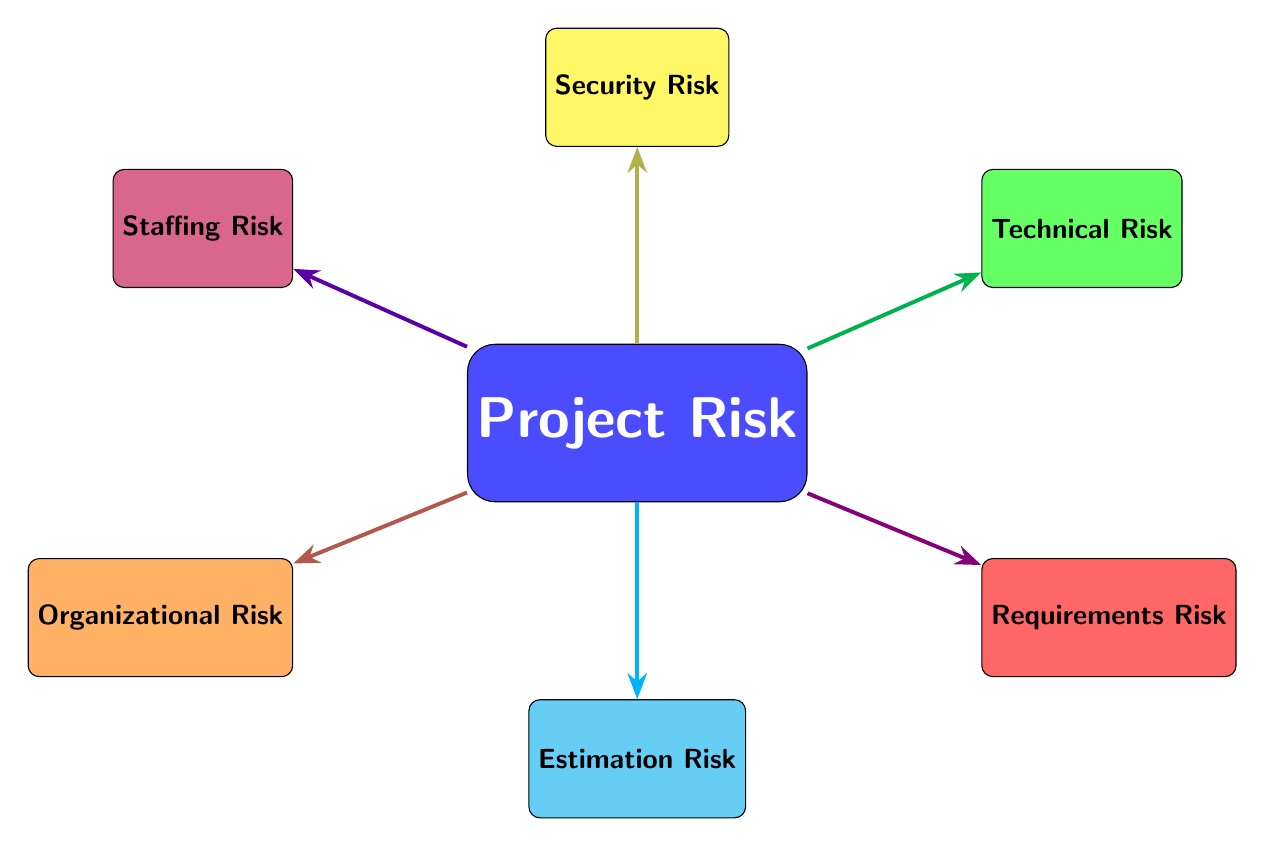
\begin{tikzpicture}[
    node distance=1cm,  % Distance between central and surrounding nodes
    every node/.style={rectangle, draw, minimum size=1.5cm, font=\sffamily\bfseries, rounded corners, text centered}, 
    arrow/.style={-Stealth, thick},  % Thicker arrows
    concept/.style={draw, rounded corners, minimum size=1.5cm, font=\sffamily\bfseries},
    ombreArrow/.style={draw, thick, -Stealth, line width=0.5mm}  % Reduced thickness of the arrows
]

    % Main Project Risk node in the center with a cloud shape
    \node (projectrisk) [fill=blue!70, text=white, minimum size=2cm, rounded corners=10pt] {\textbf{\huge Project Risk}};
    
    % Surrounding nodes (now 6 nodes, spread out somewhat symmetrically)
    \node (staffing) [above left=of projectrisk, fill=purple!60, text=black, xshift=-1.5cm] {Staffing Risk};
    \node (technical) [above right=of projectrisk, fill=green!60, text=black, xshift=1.5cm] {Technical Risk};
    \node (organizational) [below left=of projectrisk, fill=orange!60, text=black, xshift=-1.5cm] {Organizational Risk};
    \node (requirements) [below right=of projectrisk, fill=red!60, text=black, xshift=1.5cm] {Requirements Risk};
    \node (estimation) [below=of projectrisk, fill=cyan!60, text=black, yshift=-1.5cm] {Estimation Risk};
    \node (security) [above=of projectrisk, fill=yellow!60, text=black, yshift=1.5cm] {Security Risk};  
    
    % Ombre arrows 
    \draw [ombreArrow, color=blue!30!violet] (projectrisk) -- (staffing);
    \draw [ombreArrow, color=blue!30!green] (projectrisk) -- (technical);
    \draw [ombreArrow, color=blue!30!orange] (projectrisk) -- (organizational);
    \draw [ombreArrow, color=blue!30!purple] (projectrisk) -- (requirements);
    \draw [ombreArrow, color=blue!30!cyan] (projectrisk) -- (estimation);
    \draw [ombreArrow, color=blue!30!yellow] (projectrisk) -- (security); 

\end{tikzpicture}
\end{center}

\vspace{1 cm}

\pagebreak
\section{Risk Description}

As the diagram above illustrates, the project risk can be divided into six prominent areas:

\vspace{0.5cm}

\subsection{Staffing Risk}
\begin{itemize}
    \item \textbf{Quitting Members:} Team members leaving before project completion can cause delays and quality issues.
    \item \textbf{Conflicts:} Disagreements among team members can hinder collaboration and productivity.
    \item \textbf{Communication Issues:} Poor communication can lead to misunderstandings and project delays.
    \item \textbf{Different Ambitions:} Varying levels of commitment and goals among members may lead to disagreements.
    \item \textbf{Illness:} Health issues lead to unexpected absences.
\end{itemize}

\vspace{0.5cm}

\subsection{Security Risk}
\begin{itemize}
    \item \textbf{GDPR Compliance:} Non-compliance with data protection regulations can result in legal issues.
    \item \textbf{Data Breaches:} Inadequate safeguards expose sensitive information.
    \item \textbf{User Negligence:} Human error increases the risk of breaches.
\end{itemize}

\vspace{0.5cm}

\subsection{Technical Risk}
\begin{itemize}
    \item \textbf{Technology Employed:} Dependency on third-party tools that may become deprecated or unsupported.
    \item \textbf{Technical Processes:} Risk of losing critical code due to lack of version management.
    \item \textbf{Scaling Technology:} Infrastructure might fail to scale effectively under high load or multiple users.
    \item \textbf{Testing:} Limitations in testing environments may affect the ability to test all scenarios.
\end{itemize}

\vspace{0.5cm}

\subsection{Requirement Risk}
\begin{itemize}
    \item \textbf{Scope and Objectives:} Misunderstandings lead to unmet expectations.
    \item \textbf{Miscommunication:} Lack of clarity causes project delays.
    \item \textbf{Failure to Meet Expectations:} Discrepancies between deliverables and requirements.
    \item \textbf{Scope Creep:} Uncontrolled addition of features without adjusting timelines or resources.
\end{itemize}

\vspace{0.5cm}

\subsection{Estimation Risk}
\begin{itemize}
    \item \textbf{Inaccurate Time Estimates:} Underestimating time required for tasks can cause missed deadlines.
    \item \textbf{Underestimation of Complexity:} Tasks may be simpler than they seem, leading to unexpected development issues.
    \item \textbf{Insufficient Buffer:} Lack of contingency time for unexpected issues.
    \item \textbf{Lack of Task Breakdown:} Unclear tasks complicate time management.
\end{itemize}

\vspace{0.5cm}

\subsection{Organizational Risk}
\begin{itemize}
    \item \textbf{Unclear Responsibilities:} Ambiguity in roles can cause misalignment and missed deadlines.
    \item \textbf{Unclear Role Definition:} Hesitation in decision-making hampers progress.
    \item \textbf{Task Overload:} Burnout decreases productivity and morale.
    \item \textbf{Decision-Making Bottlenecks:} Delays occur when too few people make decisions.
    \item \textbf{Individual Time Tracking:} Tracking of individual effort through a common time report may be misused, leading to uneven workloads. This unfairness could cause frustration between employees. Currently, each individual must weekly report the time spent on the project each day. Since this is a manual and independent task, an employee might forget to log time or log time they haven’t actually worked.
\end{itemize}


\pagebreak

\section{Risk Analysis}
To assess risks, both probability and impact are rated on a scale from 1 to 4, with 1 denoting the lowest level and 4 the highest. The overall risk magnitude is determined by multiplying the probability by the impact, producing a value ranging from 1 to 16.
\[
\text{Risk Magnitude} = \text{Probability} \times \text{Impact}
\]

\begin{center}
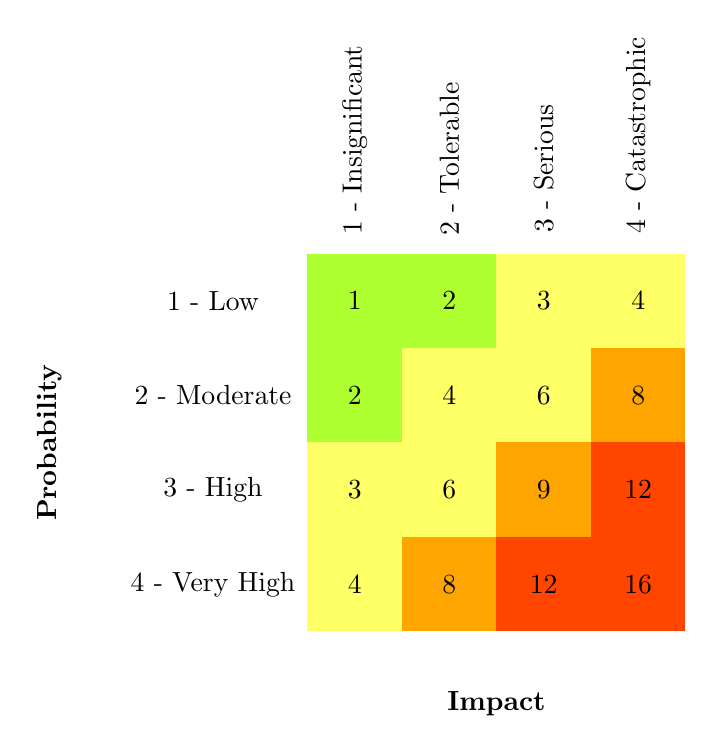
\begin{tikzpicture}[scale=1.2] % Increase the scale to give more room

% Define the colors for the risk magnitude levels
\definecolor{low}{RGB}{173, 255, 47}      % light green for low risks
\definecolor{moderate}{RGB}{255, 255, 102} % yellow for moderate risks
\definecolor{high}{RGB}{255, 165, 0}       % orange for high risks
\definecolor{critical}{RGB}{255, 69, 0}    % red for critical risks

% Probability and Impact labels
\node[anchor=south] at (3,5.-5) {\textbf{Impact}};
\node[anchor=east] at (-1.5,3) {\rotatebox{90}{\textbf{Probability}}};

% Define the columns for the table (Impact axis)
\node[rotate=90] at (1.5,6.2) {1 - Insignificant};
\node[rotate=90] at (2.5,6) {2 - Tolerable};
\node[rotate=90] at (3.5,5.9) {3 - Serious};
\node[rotate=90] at (4.5,6.25) {4 - Catastrophic};

% Define the rows for the table (Probability axis)
\node at (0,4.5) {1 - Low};
\node at (0,3.5) {2 - Moderate};
\node at (0,2.5) {3 - High};
\node at (0,1.5) {4 - Very High};



% Row 1: Low Probability
\fill[low]       (1,4) rectangle (2,5); \node at (1.5,4.5) {1};
\fill[low]       (2,4) rectangle (3,5); \node at (2.5,4.5) {2};
\fill[moderate]  (3,4) rectangle (4,5); \node at (3.5,4.5) {3};
\fill[moderate]  (4,4) rectangle (5,5); \node at (4.5,4.5) {4};

% Row 2: Moderate Probability
\fill[low]       (1,3) rectangle (2,4); \node at (1.5,3.5) {2};
\fill[moderate]  (2,3) rectangle (3,4); \node at (2.5,3.5) {4};
\fill[moderate]  (3,3) rectangle (4,4); \node at (3.5,3.5) {6};
\fill[high]      (4,3) rectangle (5,4); \node at (4.5,3.5) {8};

% Row 3: High Probability
\fill[moderate]  (1,2) rectangle (2,3); \node at (1.5,2.5) {3};
\fill[moderate]  (2,2) rectangle (3,3); \node at (2.5,2.5) {6};
\fill[high]      (3,2) rectangle (4,3); \node at (3.5,2.5) {9};
\fill[critical]  (4,2) rectangle (5,3); \node at (4.5,2.5) {12};

% Row 4: Very High Probability
\fill[moderate]  (1,1) rectangle (2,2); \node at (1.5,1.5) {4};
\fill[high]      (2,1) rectangle (3,2); \node at (2.5,1.5) {8};
\fill[critical]  (3,1) rectangle (4,2); \node at (3.5,1.5) {12};
\fill[critical]  (4,1) rectangle (5,2); \node at (4.5,1.5) {16};

\end{tikzpicture}
\end{center}


\setlength{\tabcolsep}{4pt} % Reduce column padding
\subsection{Staffing Risk}
\begin{flushleft} % Adjust alignment if needed (you can use \centering or \flushright)
    \begin{tabular}{|p{1cm}|c|p{5cm}|>{\centering\arraybackslash}p{2cm}|>{\centering\arraybackslash}p{2cm}|>{\centering\arraybackslash}p{2cm}|}
        \hline
        \textbf{Risk Name} & \textbf{\#} & \textbf{Risk Description \& Plan} & \textbf{Probability} & \textbf{Impact} & \textbf{Risk Factor} \\
        \hline
        \multirow{5}{*}{\centering\fontsize{25}{35}\selectfont\rotatebox{90}{Staffing Risk}} & 1 
        & \textbf{Quitting Members:} A project member quits the course.
        & 1 & 3 & 3 \\
        \cline{3-6} % Horizontal line for the risk plan starting from the column nr
        & & \multicolumn{4}{|p{12.5cm}|}{\colorbox{yellow}{\parbox{12.5cm}{\textbf{Contingency plan:} \hyperref[sec:contingency]{Follow the contingency plan for sick and or absent members.}}}} \\
        \cline{2-6} % Line for the next risk. för att ändra är det varannan
        & 2
        & \textbf{Communication issues:} Communication issues arise that lead to misunderstandings and project delays. 
        & 4 & 2 & 8 \\
        \cline{3-6} 
        & & \multicolumn{4}{|p{12.5cm}|}{\colorbox{orange}{\parbox{12.5cm}{\textbf{Avoid risk:} Establish clear communication channels and regular updates.}}} \\
        \cline{2-6} 
        & 3
        & \textbf{Ambition Misalignment:} Different ambitions among team members become apparent as the project proceeds.
        & 4 & 1 & 4 \\
        \cline{3-6} 
        & & \multicolumn{4}{|p{12.5cm}|}{\colorbox{yellow}{\parbox{12.5cm}{\textbf{Avoid risk:} Continuous alignment goals through regular meetings.}}} \\
        \cline{2-6} 
        & 4
        & \textbf{Risk Description:} A project member falls ill
        & 2 & 2 & 4 \\
        \cline{3-6} 
        & & \multicolumn{4}{|p{12.5cm}|}{\colorbox{yellow}{\parbox{12.5cm}{
    \textbf{Contingency plan:} \hyperref[sec:contingency]{Follow the contingency plan for sick and or absent members.}
}}}\\
        \hline
    \end{tabular}
\end{flushleft}

%%%%%%%%
%SECURITY RISK
\subsection{Security Risk}
\begin{flushleft} % Adjust alignment if needed (you can use \centering or \flushright)
    \begin{tabular}{|p{1cm}|c|p{5cm}|>{\centering\arraybackslash}p{2cm}|>{\centering\arraybackslash}p{2cm}|>{\centering\arraybackslash}p{2cm}|}
        \hline
        \textbf{Risk Name} & \textbf{\#} & \textbf{Risk Description \& Plan} & \textbf{Probability} & \textbf{Impact} & \textbf{Risk Factor} \\
        \hline
        \multirow{5}{*}{\centering\fontsize{25}{35}\selectfont\rotatebox{90}{Security Risk}} & 1 
        & \textbf{GDPR Compliance:} It has been found that GDPR regulations are not being adhered to.
        & 3 & 3 & 9 \\
        \cline{3-6} % Horizontal line for the risk plan starting from the column nr
        & & \multicolumn{4}{|p{12.5cm}|}{\colorbox{orange}{\parbox{12.5cm}{\textbf{Avoid risk:} Ensure GDPR compliance is planned for and integrated early in the project planning phase.}}} \\
        \cline{2-6} % Line for the next risk. för att ändra är det varannan
        & 2
        & \textbf{Data Breaches:} Inadequate safeguards expose sensitive information. 
        & 2 & 3 & 6 \\
        \cline{3-6} 
        & & \multicolumn{4}{|p{12.5cm}|}{\colorbox{yellow}{\parbox{12.5cm}{\textbf{Avoid risk:} Continuously prioritize robust data security measures throughout all iterations of the project. }}} \\
        \cline{2-6} 
        & 3
        & \textbf{User Negligence:} Human error causes data breach 
        & 3 & 3 & 9 \\
        \cline{3-6} 
        & & \multicolumn{4}{|p{12.5cm}|}{\colorbox{orange}{\parbox{12.5cm}{\textbf{Avoid risk:} Continuously prioritize robust data security measures throughout all iterations of the project.}}} \\
        \cline{2-6} 
        \hline
    \end{tabular}
\end{flushleft}

%%%%%%%%%%%%%%%%%%%
%TECHNICAL RISK 
%%%%%%%%%
\subsection{Technical Risk}
\begin{flushleft} % Adjust alignment if needed (you can use \centering or \flushright)
    \begin{tabular}{|p{1cm}|c|p{5cm}|>{\centering\arraybackslash}p{2cm}|>{\centering\arraybackslash}p{2cm}|>{\centering\arraybackslash}p{2cm}|}
        \hline
        \textbf{Risk Name} & \textbf{\#} & \textbf{Risk Description \& Plan} & \textbf{Probability} & \textbf{Impact} & \textbf{Risk Factor} \\
        \hline
        \multirow{5}{*}{\centering\fontsize{25}{35}\selectfont\rotatebox{90}{Technical Risk}} & 1 
        & \textbf{Technology Employed:} Third-party tools like Microsoft Planer, Microsoft AZURE, Teams become suddenly unavailable.
        & 1 & 3 & 3 \\
        \cline{3-6} % Horizontal line for the risk plan starting from the column nr
        & & \multicolumn{4}{|p{12.5cm}|}{\colorbox{yellow}{\parbox{12.5cm}{\textbf{Mitigation:} Identify a reliable third-party tool that offers comparable functionality to serve as a backup. For example, consider using Google Sheets as an alternative to Microsoft Planner.}}} \\
        \cline{2-6} % Line for the next risk. för att ändra är det varannan
        & 2
        & \textbf{Technical Processes:} Critical code is lost due to lack of version management. 
        & 3 & 3 & 9 \\
        \cline{3-6} 
        & & \multicolumn{4}{|p{12.5cm}|}{\colorbox{orange}{\parbox{12.5cm}{\textbf{Avoid risk:} Emphasize the importance of adhering to proper GitLab push and pull etiquette consistently and timely throughout all project iterations. }}} \\
        \cline{2-6} 
        & 3
        & \textbf{Scaling Technology:} Kubernetes may experience failures under heavy load or when accessed by numerous users simultaneously.
        & 3 & 4 & 12 \\
        \cline{3-6} 
        & & \multicolumn{4}{|p{12.5cm}|}{\colorbox{red}{\parbox{12.5cm}{\textbf{Mitigation:} To mitigate this risk, implement scalable infrastructure solutions, such as load balancing and cloud services, to ensure stability during peak usage times.}}} \\
        \cline{2-6} 
        & 4
        & \textbf{Testing Enviroment:} Resource and testing environment limitations may hinder scenario testing, potentially increasing program bugs.
        & 3 & 3 & 9 \\
        \cline{3-6} 
        & & \multicolumn{4}{|p{12.5cm}|}{\colorbox{orange}{\parbox{12.5cm}{\textbf{ Mitigation:} Ensuring adequate resources and diverse testing environments are available to comprehensively test all scenarios before deployment.}}} \\
        \cline{2-6} 
        \hline
    \end{tabular}
\end{flushleft}

%%%%%%%%%
%REQUIREMENT RISK
%%%%%%%%%%
\subsection{Requirement Risk}
\begin{flushleft} % Adjust alignment if needed (you can use \centering or \flushright)
    \begin{tabular}{|p{1cm}|c|p{5cm}|>{\centering\arraybackslash}p{2cm}|>{\centering\arraybackslash}p{2cm}|>{\centering\arraybackslash}p{2cm}|}
        \hline
        \textbf{Risk Name} & \textbf{\#} & \textbf{Risk Description \& Plan} & \textbf{Probability} & \textbf{Impact} & \textbf{Risk Factor} \\
        \hline
        \multirow{5}{*}{\centering\fontsize{25}{35}\selectfont\rotatebox{90}{Requirement Risk}} & 1 
        & \textbf{Scope and Objectives} Miscommunication and misunderstanding between analysts and stakeholders and analysts and developers.
        & 2 & 3 & 6 \\
        \cline{3-6} % Horizontal line for the risk plan starting from the column nr
        & & \multicolumn{4}{|p{12.5cm}|}{\colorbox{yellow}{\parbox{12.5cm}{\textbf{Avoid risk:} Establish regular communication channels and collaborative meetings among analysts, stakeholders, and developers to ensure clarity and alignment throughout the project. Work iterative and adhere to agile methodology}}} \\
        \cline{2-6} % Line for the next risk. för att ändra är det varannan
        & 2
        & \textbf{Failure to Meet Expectations:} Stakeholder expectations are not met. 
        & 3 & 4 & 12 \\
        \cline{3-6} 
        & & \multicolumn{4}{|p{12.5cm}|}{\colorbox{red}{\parbox{12.5cm}{\textbf{Avoid risk:} Set clear objectives and performance metrics from the outset, and regularly review progress in accordance with the software requirement specification (SRS) to ensure alignment with expectations.}}} \\
        \cline{2-6} 
        & 3
        & \textbf{Scope Creep:} Expansion of project scope beyond original plans.
        & 2 & 3 & 6\\
        \cline{3-6} 
        & & \multicolumn{4}{|p{12.5cm}|}{\colorbox{yellow}{\parbox{12.5cm}{\textbf{Mitigation:} Establish a strict change control process to evaluate and approve any modifications to the project scope, ensuring that all stakeholders are aligned and that impacts on timelines and resources are assessed.}}} \\
        \cline{2-6} 
        \hline
    \end{tabular}
    \end{flushleft}

%%%%%%%%%
%ESTIMATION RISK
%%%%
\subsection{Estimation Risk}
\begin{flushleft} % Adjust alignment if needed (you can use \centering or \flushright)
    \begin{tabular}{|p{1cm}|c|p{5cm}|>{\centering\arraybackslash}p{2cm}|>{\centering\arraybackslash}p{2cm}|>{\centering\arraybackslash}p{2cm}|}
        \hline
        \textbf{Risk Name} & \textbf{\#} & \textbf{Risk Description \& Plan} & \textbf{Probability} & \textbf{Impact} & \textbf{Risk Factor} \\
        \hline
        \multirow{5}{*}{\centering\fontsize{25}{35}\selectfont\rotatebox{90}{Estimation Risk}} & 1 
        & \textbf{Underestimation of Complexity and Time Estimates:} Tasks take more time than initially thought and are more complex
        & 3 & 4 & 12 \\
        \cline{3-6} % Horizontal line for the risk plan starting from the column nr
        & & \multicolumn{4}{|p{12.5cm}|}{\colorbox{red}{\parbox{12.5cm}{\textbf{Avoid risk:} Conduct a detailed requirements analysis and engage in iterative reviews with stakeholders to refine complexity assessments and time estimates, ensuring that potential challenges are identified and addressed early in the project.}}} \\
        \cline{2-6} % Line for the next risk. för att ändra är det varannan
        & 2
        & \textbf{Insufficient Buffer} Lack of slack time for unexpected issues
        & 3 & 3 & 9 \\
        \cline{3-6} 
        & & \multicolumn{4}{|p{12.5cm}|}{\colorbox{orange}{\parbox{12.5cm}{\textbf{Avoid risk:} Implement a planning strategy that includes building in a sufficient buffer for both time and resources, allowing flexibility to accommodate unforeseen issues without jeopardizing project timelines.}}} \\
        \cline{2-6} 
        & 3
        & \textbf{Lack of Task Breakdown:} Unclear tasks as iterations proceed
        & 3 & 3 & 9 \\
        \cline{3-6} 
        & & \multicolumn{4}{|p{12.5cm}|}{\colorbox{orange}{\parbox{12.5cm}{\textbf{Avoid risk:} Ensure a comprehensive task breakdown by creating a detailed work breakdown structure (WBS) that outlines each task, its dependencies, and the responsible parties, facilitating better planning and tracking of project progress.}}} \\
        \cline{2-6}
        \hline
    \end{tabular}
    \end{flushleft}

%%%%%%%%%
%ORGANIZATIONAL RISK
%%%%%%%%
\subsection{Organizational Risk}
\begin{flushleft} % Adjust alignment if needed (you can use \centering or \flushright)
    \begin{tabular}{|p{1cm}|c|p{5cm}|>{\centering\arraybackslash}p{2cm}|>{\centering\arraybackslash}p{2cm}|>{\centering\arraybackslash}p{2cm}|}
        \hline
        \textbf{Risk Name} & \textbf{\#} & \textbf{Risk Description \& Plan} & \textbf{Probability} & \textbf{Impact} & \textbf{Risk Factor} \\
        \hline
        \multirow{5}{*}{\centering\fontsize{25}{35}\selectfont\rotatebox{90}{Organizational Risk}} & 1 
        & \textbf{Unclear Roll Definitions and Responsibites:} Unclear role definitions and responsibilities due to cross functional teams that lead to overlap in tasks, and missed deadlines.
        & 1 & 2 & 2 \\
        \cline{3-6} % Horizontal line for the risk plan starting from the column nr
        & & \multicolumn{4}{|p{12.5cm}|}{\colorbox{green}{\parbox{12.5cm}{\textbf{Avoid risk:} Establish clear role definitions and responsibilities through regular status reports and follow up meetings.}}} \\
        \cline{2-6} % Line for the next risk. för att ändra är det varannan
        & 2
        & \textbf{Task Overload} Project member(s) are assigned too many responsibilities, leading to decreased productivity, increased stress, and a higher likelihood of errors. 
        & 3 & 3 & 9 \\
        \cline{3-6} 
        & & \multicolumn{4}{|p{12.5cm}|}{\colorbox{orange}{\parbox{12.5cm}{\textbf{Avoid risk:} Implement workload management practices by regularly assessing team capacity, prioritizing tasks, and redistributing work as necessary to ensure a balanced workload for all project members.}}} \\
        \cline{2-6} 
        & 3
        & \textbf{Decision-Making Bottleneck:} Critical decisions are delayed due to Project Manager absence, Architect absence or lack of clear processes. 
        & 1 & 4 & 4 \\
        \cline{3-6} 
        & & \multicolumn{4}{|p{12.5cm}|}{\colorbox{yellow}{\parbox{12.5cm}{\textbf{Avoid risk:} Establish clear decision-making protocols, delegate authority appropriately, and empower team members to make decisions within their areas of responsibility to streamline the decision-making process and prevent bottlenecks.}}} \\
        \cline{2-6} 
        & 3
        % Time tracking:
        & \textbf{Individual Time Tracking:} Tracking of individual effort through a common time report may be (purposely or involuntarily) misused, which enables uneven workloads to exist within the company. 
        & 3 & 3 & 9 \\
        \cline{3-6} 
        & & \multicolumn{4}{|p{12.5cm}|}{\colorbox{orange}{\parbox{12.5cm}{\textbf{Avoid risk:} Establish clear guidelines for individual reporting of time, including what to report, when to report, how to report, and why each individual is obliged to report their time. Furthermore, both the total time spent for each employee and a burn-down chart for the company's time is available in the same excel as the Time Report, with the aim to encourage employee to match their effort to that of the rest of the company.}}} \\
        \cline{2-6} 
        \hline
    \end{tabular}
    \end{flushleft}

\newpage
\section{Risk Planning}

The Risk Planning details proactive strategies for managing identified risks throughout the project. By implementing these measures, the project aims to minimize potential disruptions and ensure successful outcomes. Among the various risks we face, employee sickness stands out as one of the most significant. This underscores the necessity of having a robust contingency plan in place, ensuring that we can adapt and respond effectively to any health-related challenges that may arise.

\subsection{Contingency Plan}
\label{sec:contingency}
\begin{enumerate}[label=\textbf{\arabic*.}]
    \item The project member should contact their direct manager or project manager as soon as possible, preferably before their shift starts.  

    \item The direct manager or project manager notes the project member's name, date of notification, and reason for absence.  

    \item The direct manager or project manager assesses the project member’s current workload and identifies tasks that need immediate attention.  

    \item Assign the project member's tasks to other team members to ensure work continues without major disruptions.  

    \item Notify the team about the project member’s absence and the temporary redistribution of their duties without disclosing personal details. If necessary, inform the CEO or examiner of any changes or delays.  

    \item Remind the project member to focus on their health and recovery. Share information about health resources or employee assistance programs.  

    \item After a few days, the direct manager or project manager should reach out to see how the project member is feeling and discuss their return to work.  

    \item Ensure the project member is fit to return before they come back. 

    \item After the project member returns, discuss what went well and what could be improved in the response to their absence.  
\end{enumerate}

Apart from risks related to illness, the strategies for the previously mentioned risks are as follows:

\newpage
\section{Risk Monitoring}

Ongoing evaluation and monitoring of risks will be conducted to ensure that mitigation strategies are effective and to address new risks as they emerge throughout the project lifecycle.

IMAGINE A TABLE ABOUT CURRENT RISKS


\subsection{Measurement of Individual Time Tracking: }
On each Manager meeting, held on Monday lunch, the Project Manager and the Line Managers follow up the past weeks hours spent on the project and compare different groups, teams, and individual situations, to assess if the time spent is fair and in accordance to the expectations for that time frame. Th Process Manager has therefore constructed individual burn-down charts for each employee. 

After the Pre-Study phase and Iteration 1 it is clear that some groups have spent more time on the project, especially the Managers and the Analysts. However, this is to be expected as groups, such as, Developers and Testers have tasks more prominent in later iterations.

\begin{figure}[h]
    \centering
    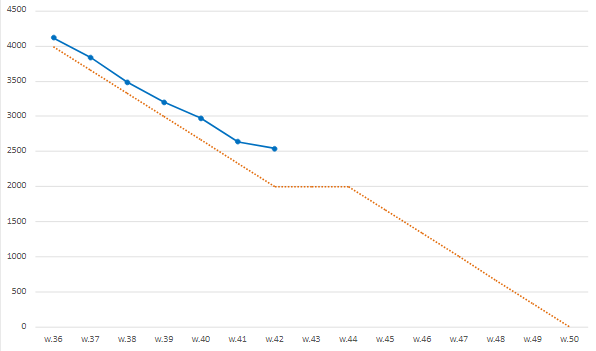
\includegraphics[width=0.5\linewidth]{2024-10-16.png}
    \caption{Burn-down chart for Comapny 3 after Iteration 1}
    \label{fig:enter-label}
\end{figure}


\end{document}



\begin{figure}[h]
    \centering
    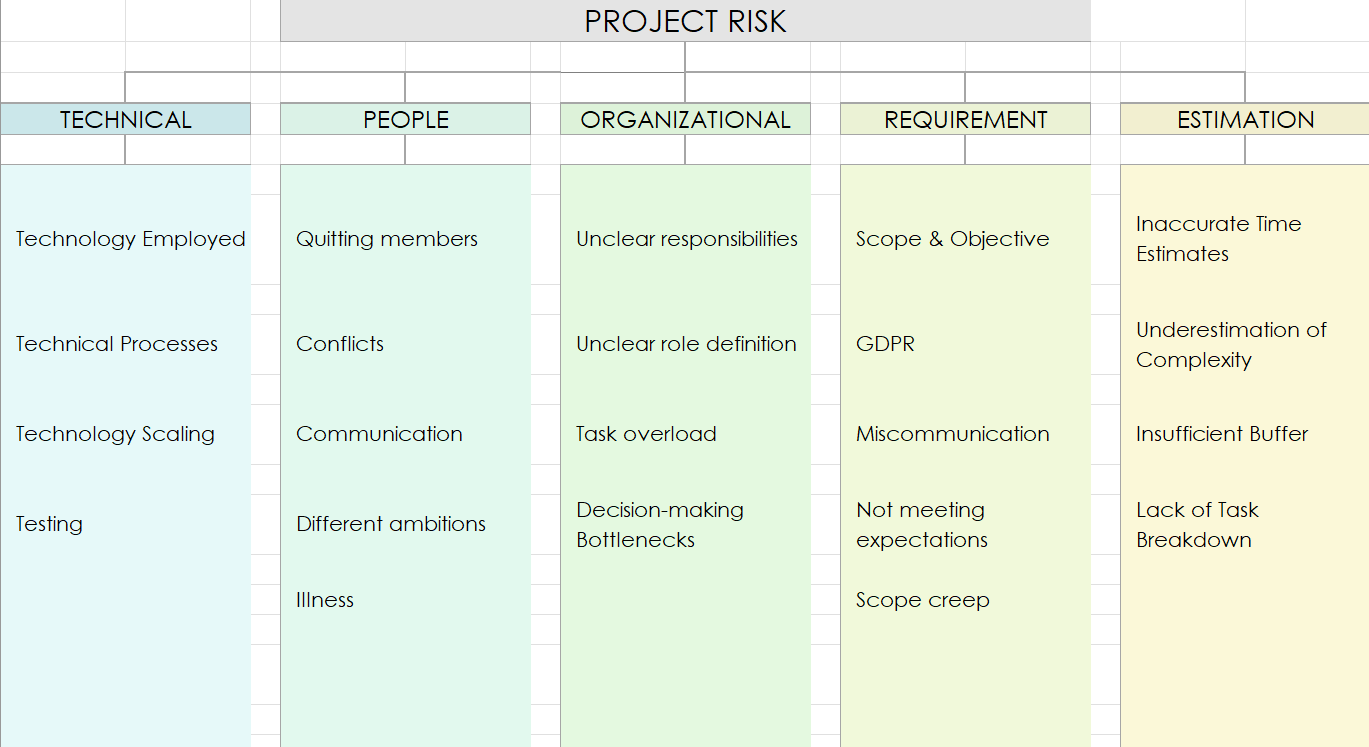
\includegraphics[width=1.0\linewidth]{Risk Diagram List.png}
    \caption{Risk Breakdown Structure}
    \label{fig:enter-label}
\end{figure}



The following table provides detailed descriptions of each identified risk, outlining their potential causes and specific impacts on the project to support further analysis and mitigation efforts.

\begin{table}[h]
\centering
\begin{tabularx}{\linewidth}{|l|X|}
\hline
\multicolumn{1}{|c|}{\textit{\textbf{Risks}}} & \multicolumn{1}{c|}{\textit{\textbf{Risks Description}}}                                                   \tabularnewline \hline
 Technology Employed & Dependency on third-party tools that may become deprecated or unsupported.\tabularnewline \hline
 Technical Processes & Risk of losing critical code due to lack of version management.\tabularnewline \hline
 Technology Scaling & Infrastructure might fail to scale effectively under high load or multiple users.\tabularnewline \hline
 Testing & Limitations in testing environments may affect the ability to test all scenarios.\tabularnewline \hline
 Quitting Members & Team members leaving before project completion can cause delays and quality issues.\tabularnewline \hline
 Conflicts & Disagreements among team members can hinder collaboration and productivity.\tabularnewline \hline
 Communication & Poor communication can lead to misunderstandings and project delays.\tabularnewline \hline
 Different Ambitions & Varying levels of commitment and goals among members may lead to disagreements.\tabularnewline \hline
 Unclear Responsibilities & Ambiguity in roles can cause misalignment and missed deadlines.\tabularnewline \hline
 Scope Creep & Uncontrolled addition of features without adjusting timelines or resources.\tabularnewline \hline
 GDPR & Non-compliance with data protection regulations can result in legal issues.\tabularnewline \hline
 Inaccurate Time Estimates & Underestimating time required for tasks can cause missed deadlines.\tabularnewline \hline
 Underestimation of Complexity & Tasks may be simpler than they seem, leading to unexpected development issues.\tabularnewline \hline

\end{tabularx}
\caption{Risks identified in the project.}
\label{table:risks}   
\end{table}
\pagebreak
</main.tex>


</COMPILED_DOCUMENT>

Generate the LaTeX-formatted change history table based on the provided INSTRUCTIONS, README_CONTENT, and COMPILED_DOCUMENT. Use your understanding of the project context to create an informative and well-structured change history. Ensure that the output is properly formatted and ready to be included in a LaTeX document.
  